\documentclass[aspectratio=169]{beamer}
\usepackage{pgf}
\usepackage{multimedia}
\usepackage{colortbl,tabularx,mathrsfs,calligra,xcolor}
\usepackage{amsmath,amsfonts,amssymb,amsthm}
\usepackage{ragged2e}
\usepackage{setspace}
\usepackage{filecontents}
\usepackage{caption}
\usepackage{subcaption}
\usepackage{contour}
\usepackage{animate}
\usepackage{fancybox}
\usepackage{wrapfig}
\usepackage{multirow}
\usepackage{multicol}
\usepackage{pgfplots, tkz-euclide,calc}
    \usetikzlibrary{patterns,snakes,shapes.arrows,shapes.geometric,arrows}
\usepackage{listings}
\usepackage{enumitem}
\usepackage{pifont}
\usepackage[scaled]{berasans}
    \renewcommand*\familydefault{\sfdefault}  %% Only if the base font of the document is to be sans serif
\usepackage[T1]{fontenc}
\usepackage{hyperref}
\hypersetup{
    filecolor=magenta,      
    urlcolor=cyan,
    pdftitle={Overleaf Example},
    pdfpagemode=FullScreen,
    }
\renewcommand*\familydefault{\sfdefault} %% Only if the base font of the document is to be sans serif

\graphicspath{{C:/Users/teoso/OneDrive/Documents/Asisten Dosen & Lab/Asisten Laboratorium/Alpro 1/PPT/Graphicx/}}

\definecolor{HIMAmuda}{HTML}{01D1FD}
\definecolor{HIMAtua}{HTML}{02016A}
\definecolor{HIMAabu}{HTML}{CBCBCC}
\definecolor{PastelGreen}{HTML}{77DD77}
\definecolor{pgray}{rgb}{0.5,0.5,0.5}
\definecolor{pblue}{rgb}{0.13,0.13,1}
\definecolor{pgreen}{rgb}{0,0.5,0}
\definecolor{pred}{rgb}{0.9,0,0}
\definecolor{pgrey}{rgb}{0.46,0.45,0.48}
\definecolor{pcyan}{HTML}{D4EFFC}
\definecolor{lblue}{HTML}{00AEEF}
\definecolor{input}{HTML}{AAE1FA}
\definecolor{bg}{rgb}{0.95, 0.95, 0.92}
\definecolor{vscode}{HTML}{282A36}

\usetheme{Madrid}

\setbeamercolor{palette primary}{bg=HIMAtua,fg=white}
\setbeamercolor{palette secondary}{bg=HIMAmuda,fg=black}
\setbeamercolor{palette tertiary}{bg=HIMAabu,fg=black}
\setbeamercolor{palette quaternary}{bg=HIMAmuda,fg=white}
\setbeamercolor{structure}{fg=HIMAmuda} % itemize, enumerate, etc
\setbeamercolor{section in toc}{fg=HIMAtua} % TOC sections
\setbeamercolor{block title alerted}{fg=white,bg=magenta}
\setbeamercolor{block body alerted}{fg=black!90,bg=pink}

\usefonttheme{professionalfonts}
\setbeamertemplate{theorems}[numbered]
\setbeamertemplate{itemize items}[circle]

\usebackgroundtemplate{%
\tikz[overlay,remember picture] \node[opacity=0.1, at=(current page.center)]{\includegraphics[width=\paperwidth]{plana class}};
}

\renewcommand\thesubfigure{\arabic{subfigure}}
\newtheorem*{funfact}{Fun Fact}
\newtheorem{latihan}{Latihan}
\newtheorem*{definisi}{Definisi}
\newtheorem{teorema}{Teorema}
\theoremstyle{definition}
\newtheorem*{contoh}{Contoh}
\newtheorem*{masalah}{Masalah}
\newcommand{\R}{\mathbb{R}}

\AtBeginEnvironment{contoh}{%
    \setbeamercolor{block title}{use=example text,fg=white,bg=example text.fg!75!black}
    \setbeamercolor{block body}{parent=normal text,use=block title example,bg=block title example.bg!10!bg}
}

\AtBeginEnvironment{funfact}{%
  \setbeamercolor{block title}{fg=white,bg=PastelGreen!50!HIMAmuda} % Set title background to pastel green and text to white
  \setbeamercolor{block body}{parent=normal text,bg=PastelGreen!50!HIMAmuda!30!white} % Set body background to a lighter pastel green
}
\AtBeginEnvironment{definisi}{
    \setbeamercolor{block title}{fg=white,bg=HIMAtua}
    \setbeamercolor{block body}{parent=normal text,bg=HIMAtua!30!white}
}
\AtBeginEnvironment{teorema}{
    \setbeamercolor{block title}{bg=darkgray,fg=white}
    \setbeamercolor{block body}{parent=pallette tertiary,bg=HIMAabu!30!white}
}
\AtBeginEnvironment{latihan}{%
  \setbeamercolor{block title}{fg=white,bg=PastelGreen} % Set title background to pastel green and text to white
  \setbeamercolor{block body}{parent=normal text,bg=PastelGreen!30!white} % Set body background to a lighter pastel green
}
\AtBeginEnvironment{masalah}{%
  \setbeamercolor{block title}{fg=white,bg=teal} % Set title background to pastel green and text to white
  \setbeamercolor{block body}{parent=normal text,bg=teal!30!white} % Set body background to a lighter pastel green
}

\renewcommand{\arraystretch}{1.3}

\usepackage{listings}

\lstdefinestyle{standard}{
    language            = Java,
    showspaces          = false,
    showtabs            = false,
    breaklines          = true,
    showstringspaces    = false,
    breakatwhitespace   = true,
    commentstyle        = \color{pgray},
    keywordstyle        = \color{pblue},
    stringstyle         = \color{pgreen},
    basicstyle          = \footnotesize\ttfamily,
    frame               = shadowbox,
    backgroundcolor     = \color{brown!10!white},
    escapeinside        = {(*}{*)},
    numbers             = left, % {none, left, right}
    numberstyle         = \scriptsize\color{lightgray},
    numbersep           = -8pt,
    rulesepcolor        =\color{brown!50!black}
    }

\lstdefinestyle{output}{
    language=Java,
    backgroundcolor     =\color{vscode},
    basicstyle          =\footnotesize\ttfamily\color{white},
    frame               =shadowbox,
    escapeinside        ={(*}{*)},
    showspaces          =false,
    showtabs            =false,
    breaklines          =true,
    showstringspaces    =false,
    breakatwhitespace   =true,
    rulesepcolor        =\color{HIMAtua!50!white},
    rulecolor           =\color{HIMAtua!50!white},
    numbers             =none,
    }

\lstset{style=standard}

\tikzstyle{startstop} = [rectangle, rounded corners, 
minimum width=2cm, 
minimum height=1cm,
text centered, 
draw=black, 
fill=pink]

\tikzstyle{io} = [trapezium, 
trapezium stretches=true, % A later addition
trapezium left angle=70, 
trapezium right angle=110, 
minimum width=2cm, 
minimum height=1cm, text centered, 
draw=black, fill=HIMAmuda]

\tikzstyle{process} = [rectangle, 
minimum width=2cm, 
minimum height=1cm, 
text centered, 
text width=2cm, 
draw=black, 
fill=HIMAabu]

\tikzstyle{decision} = [diamond, 
minimum width=2cm, 
minimum height=1cm, 
text centered, 
draw=black, 
fill=PastelGreen]
\tikzstyle{arrow} = [thick,->,>=stealth]

\newcommand{\enter}{\raisebox{-1.8pt}{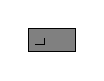
\begin{tikzpicture}[scale=0.3]
    \draw[thin,fill=gray] (0,0) rectangle (2,1);
    \draw (0.3,0.3) -- (0.7,0.3)--(0.7,0.6);     
\end{tikzpicture}}}

\newcommand{\inputscan}[1]{\raisebox{0pt}[1pt]{\colorbox{darkgray}{#1}}}

\newcommand{\inlineitem}{%
\leavevmode\usebeamertemplate{itemize item}
}

\author[Tew \& Haf]{Hafidz Mulia\\Teosofi Hidayah Agung}
\date{21 Oktober 2024}
\title[Alpro 1 - Week 6]{Control Flow}
\institute[Matematika ITS]{Departemen Matematika\\ Institut Teknologi Sepuluh Nopember}
\titlegraphic{{\includegraphics[scale=0.02]{M.png}$\quad$\includegraphics[scale=0.2]{Provicom.png}}}

\begin{document}
    {\usebackgroundtemplate{
        \tikz[overlay,remember picture] \node[opacity=0.2, at=(current page.center)]{\includegraphics[width=\paperwidth]{bg_2}};}
    \begin{frame}
        \titlepage
    \end{frame}
    }

    \AtBeginSection{
    {\usebackgroundtemplate{
     \tikz[overlay,remember picture] \node[opacity=0.1, at=(current page.center)]{\includegraphics[width=\paperwidth]{Java code}};}
    \begin{frame}{Daftar isi}
        \tableofcontents[currentsection]
        \begin{tikzpicture}[overlay, remember picture] 
            \node at ([yshift=.5cm]current page.south east) [
                anchor = south east, 
                ] {
            \animategraphics[autoplay,loop,width=0.2\textwidth]{30}{Arisu Dance/Arisu Dance-}{0}{186}
            };
        \end{tikzpicture}
    \end{frame}}
    }

    \begin{frame}
        \begin{masalah}
            Dalam hidup, penting untuk memahami kapan waktunya berhenti, melanjutkan, atau mengulang kembali ke titik awal. Hal tersebut perlu kita lakukan untuk mengontrol setiap langkah yang kita ambil. Jangan sampai kita terjebak dalam lingkaran yang sama atau bahkan tidak tahu kapan harus melangkah ke jalan yang benar.
        \end{masalah}
    \end{frame}

    \section{Break}
    \begin{frame}[fragile]
        \frametitle{\insertsection}
        \begin{definisi}
            \textbf{Break} adalah sebuah perintah yang digunakan untuk menghentikan atau keluar dari sebuah perulangan atau \textit{switch-case} yang sedang berjalan. Biasanya \texttt{break} berada dalam \texttt{if} atau \texttt{else} jika di dalam perulangan.
        \end{definisi}
        \begin{lstlisting}[style=standard,firstnumber=34,caption={Contoh penggunaan \texttt{break} dalam \texttt{for}}]
    for (...) {
        ...
        if (...)
            break; // Keluar dari loop
        ...
    }
        \end{lstlisting}
    \end{frame}

    \begin{frame}[fragile]
        \frametitle{\insertsection}
        \begin{contoh}
            Program untuk menentukan bilangan prima atau bilangan komposit.
        \end{contoh}
        \begin{lstlisting}[firstnumber=3]
    int bilangan = input.nextInt();
    for (int i = 2; i < bilangan; i++) {
        if (bilangan % i == 0) {
            System.out.println(bilangan + " bukan bilangan prima");
            break;
        }
        if (i == bilangan - 1)
            System.out.println(bilangan + " adalah bilangan prima");
    }
    System.out.println("Program selesai");
        \end{lstlisting}
        \begin{lstlisting}[style=output]
    Masukkan bilangan: (*\inputscan{21} \enter*)
    21 bukan bilangan prima
    Program selesai
        \end{lstlisting}
    \end{frame}

    \begin{frame}[fragile]
        \frametitle{\insertsection}
        \framesubtitle{Labeled Break}
        \begin{block}{Label}
            Label adalah sebuah penanda yang diletakkan di suatu baris pada kode program yang berfungsi sebagai penanda untuk suatu blok kode tertentu. Label digunakan untuk mengidentifikasi blok kode yang akan diekseskusi oleh perintah \texttt{break} atau \texttt{continue}.
        \end{block}
        \begin{lstlisting}[style=standard,firstnumber=9,caption={Labeled Break}]
    outerloop:
    for (...) {
        for (...) {
            if (...) {
                ...
                break outerloop; // Keluar dari semua loop di bawah label
            }
        }
    }
        \end{lstlisting}
    \end{frame}

    \begin{frame}
        \frametitle{\insertsection}
        \framesubtitle{Labeled Break}
        \begin{alertblock}{Perbedaan}
            \texttt{break} biasa hanya akan menghentikan satu perulangan saja, sedangkan \texttt{break} dengan label akan menghentikan perulangan yang diberi label (Bisa lebih dari satu perulangan, tergantung pada berapa perulangan yang berada dibawah label tersebut).
        \end{alertblock}
    \end{frame}

    \begin{frame}[fragile]
        \frametitle{\insertsection}
        \framesubtitle{Labeled Break}
        \begin{lstlisting}[firstnumber=70,caption={Non-Labeled Break}]
    for (int i = 0; i < 3; i++) {
        for (int j = 0; j < 3; j++) {
            if (j == 1) {
                break; // Hanya menghentikan loop bagian dalam
            }
            System.out.println("i = " + i + ", j = " + j);
        }
    }
        \end{lstlisting}
        \begin{lstlisting}[style=output]
    i = 0, j = 0
    i = 1, j = 0
    i = 2, j = 0
        \end{lstlisting}
    \end{frame}

    \begin{frame}[fragile]
        \frametitle{\insertsection}
        \framesubtitle{Labeled Break}
        \begin{lstlisting}[firstnumber=83,caption={Labeled Break}]
    outerLoop: // Label untuk loop luar
    for (int i = 0; i < 3; i++) {
        for (int j = 0; j < 3; j++) {
            if (j == 1) {
                break outerLoop; // Menghentikan loop luar
            }
            System.out.println("i = " + i + ", j = " + j);
        }
    }
        \end{lstlisting}
        \begin{lstlisting}[style=output]
    i = 0, j = 0
        \end{lstlisting}
    \end{frame}

    \section{Continue}
    \begin{frame}[fragile]
        \frametitle{\insertsection}
        \begin{definisi}
            \textbf{Continue} adalah sebuah perintah yang digunakan untuk melanjutkan perulangan berikutnya tanpa mengeksekusi kode di bawahnya. Berbeda dengan \texttt{break}, \texttt{continue} hanya memberhentikan atau melompati 1 iterasi saja. Program akan tetap berjalan hingga salah satu kondisi untuk berhenti terpenuhi.
        \end{definisi}
        \begin{lstlisting}[style=standard,firstnumber=59,caption={Contoh penggunaan \texttt{continue} dalam \texttt{for}}]
    for (...) {
        ...
        if (...)
            continue; // Melanjutkan ke iterasi berikutnya
        ...
    }
        \end{lstlisting}
    \end{frame}

    \begin{frame}[fragile]
        \frametitle{\insertsection}
        \begin{contoh}
            Program untuk menampilkan faktor dari sebuah bilangan.
        \end{contoh}
        \begin{lstlisting}
    int bilangan = input.nextInt();
    for (int i = 1; i <= bilangan; i++) {
        if (bilangan % i != 0)
            continue;
        System.out.print(i+" ");
    }
    System.out.println("\nProgram selesai");
        \end{lstlisting}
        \begin{lstlisting}[style=output]
    Masukkan bilangan: (*\inputscan{12} \enter*)
    1 2 3 4 6 12
    Program selesai
        \end{lstlisting}
    \end{frame}

    \begin{frame}[fragile]
        \frametitle{\insertsection}
        \framesubtitle{Labeled Continue}
        \begin{block}{Label}
            Sama seperti \texttt{break}, \texttt{continue} juga bisa diberi label. Namun, penggunaan \texttt{continue} dengan label tidak terlalu umum.
        \end{block}
        \begin{lstlisting}[style=standard,firstnumber=9,caption={Labeled Continue}]
    outerLoop: // Label untuk loop luar
    for (int i = 0; i < 3; i++) {
        for (int j = 0; j < 3; j++) {
            if (j == 1) {
                continue outerLoop; // Melompat ke iterasi berikutnya dari loop luar (i)
            }
            System.out.println("i = " + i + ", j = " + j);
        }
    }
        \end{lstlisting}
    \end{frame}

    \section{Return}
    \begin{frame}
        \frametitle{\insertsection}
        \begin{definisi}
            \textbf{Return} adalah sebuah perintah yang digunakan untuk mengembalikan nilai atau menghentikan proses dari suatu fungsi. Karena kita masih belum membahas fungsi/method, intinya return digunakan untuk menghentikan semua proses yang ada di dalam method \texttt{main} (untuk sekarang).
        \end{definisi}
    \end{frame}

    \begin{frame}[fragile]
        \frametitle{\insertsection}
        \begin{lstlisting}[firstnumber=3,caption={Contoh penggunaan \texttt{return}}]
    public static void main(String[] args) {
        int x = input.nextInt();
        if (x % 2 == 0) {
            System.out.println("Bilangan genap");
            return;
        }
        System.out.println("Bilangan ganjil");
    }
        \end{lstlisting}
        \begin{lstlisting}[style=output]
    Masukkan bilangan: (*\inputscan{12} \enter*)
    Bilangan genap
        \end{lstlisting}
        \begin{lstlisting}[style=output]
    Masukkan bilangan: (*\inputscan{7} \enter*)
    Bilangan ganjil
        \end{lstlisting}
    \end{frame}

    \section{Latihan}
    \begin{frame}
        \begin{latihan}
            Program yang menerima inputan kata sandi dari user. Jika kata sandi yang dimasukkan benar, maka program akan menampilkan "Kata sandi benar" dan berhenti. Jika kata sandi yang dimasukkan salah, maka program akan menampilkan "Kata sandi salah" dan meminta inputan kata sandi kembali. Program akan terus berjalan hingga maksimal 3 kali kesempatan untuk memasukkan kata sandi.
        \end{latihan}
    \end{frame}

    \begin{frame}
        \begin{latihan}
            Diberikan bilangan bulat random $p$ yang termuat pada interval $[-50,100]$. Buatlah program yang menerima input tebakan dari user dan akan berhenti jika tebakan benar. Jika tebakan salah, maka akan ada dua kondisi berikut:
            \begin{itemize}[label=$\triangleright$]
                \item Jika tebakan berjarak lebih dari 10 angka dari $p$, maka program akan menampilkan "Tebakan salah".
                \item Jika tebakan berada di interval $[p-10,p+10]$, maka program akan menampilkan "Tebakan hampir benar".
            \end{itemize}
            Program akan terus berjalan hingga tebakan benar dan tak ada batas maksimal percobaan. (Petunjuk: Gunakan \texttt{Math.Random()} untuk menghasilkan bilangan random).
        \end{latihan}
    \end{frame}
        
\end{document}